\documentclass[12pt]{article}

\usepackage[spanish]{babel}

\usepackage{amsmath}
\usepackage{amssymb}

\usepackage{hyperref}
\usepackage{graphicx}
\usepackage{listings}
\usepackage{color}
\usepackage{multicol}
\usepackage{enumitem}
\usepackage{here}
\usepackage{dsfont}
\usepackage{tipa}
\usepackage{float}
\usepackage{dsfont} 
\spanishdecimal{.}

\title{Matemáticas para las Ciencias Aplicadas II}
\title{
	\textbf{Tarea 02} \\
	\vspace{1ex}
	\large Matemáticas para las Ciencias Aplicadas II \\
	Facultad de Ciencias, UNAM}
\date{\today}
\author{Flores Morán Julieta Melina \\ Zarco Romero José Antonio}

\begin{document}
\maketitle

% 1 -------------------------------------------------------------------------------------------------------------
\section{}
Proporcione el dominio de la función vectorial.
\[
\vec{r(t)}
=
\frac{t-2}{t+2}\hat{i}
+
\sin{t}\hat{j}
+
\ln{(9-t^2)}\hat{k}
\]

El dominio de cada \textit{función componente} es como sigue:
\begin{itemize}[format=\textbf]

\item $f(t)=\frac{t-2}{t+2}$
  $$\left\{t \in \mathbb{R} ~|~ t \neq -2 \right\}$$

\item $g(t)=\sin{t}$
  $$\left\{t\in \mathbb{R} \right\}$$

\item $h(t)=\ln{(9-t^2)}$
  $$\left\{t\in \mathbb{R} ~|~ -3 < t < 3 \right\}$$

\end{itemize}
La intersección de los 3 conjuntos es $\left\{t\in \mathbb{R} ~|~ (-3<t<-2) ~ \land ~ (-2<t<3) \right\}$.

$\therefore$ El dominio de la función vectorial $\vec{r(t)}$ es $(-3,-2)$ \cup $(-2,3)$.


% 2 -------------------------------------------------------------------------------------------------------------
\section{}
Sea
\[
\vec{r(t)}
=
\frac{t^2-t}{t-1}\hat{i}
+
\sqrt{t+8}\hat{j}
+
\frac{\sin{\pi t}}{\ln{t}}\hat{k}
\]
Calcule $ \lim_{t \to 0} \vec{r(t)} $.

Recordemos que el límite de una función vectorial se define obteniendo los límites de sus \textit{funciones componentes}:
\begin{itemize}[format=\textbf]

\item $f(t)=\frac{t^2-t}{t-1}$
  \begin{align*}
    \lim_{t \to 0} f(t) = \lim_{t \to 0} \frac{t^2-t}{t-1}  =  \frac{0}{-1}= 0
  \end{align*}

\item $g(t)=\sqrt{t+8}$
  \begin{align*}
    \lim_{t \to 0} g(t) = \lim_{t \to 0} \sqrt{t+8} = \sqrt{8} = 2\sqrt{2}
  \end{align*}

\item $h(t)=\frac{\sin{\pi t}}{\ln{t}}$
  \begin{align*}
    \lim_{t \to 0} h(t)
    &= \lim_{t \to 0} \frac{\sin{(\pi t)}}{\ln{t}} \\
    &= \lim_{t \to 0} \frac{\frac{d}{dt} \sin{(\pi t)}}{ \frac{d}{dt} \ln{t}} \\
    &= \lim_{t \to 0} \frac{\cos{(\pi t)} \frac{d}{dt}(\pi t) }{ \frac{1}{t} } \\
    &= \lim_{t \to 0} \frac{\pi \cos{(\pi t)}}{ \frac{1}{t} } \\
    &= \lim_{t \to 0} \pi t \cos{(\pi t)} \\
    &= \pi 0 \cos{(\pi 0)} \\
    &= 0 \cdot 1 \\
    &= 0
  \end{align*}

  Según la definición, el límite de $\vec{r(t)}$ es el vector cuyas componentes son los límites de las funciones componentes de $r$, siempre y cuando existan. Entonces:
  \[
 \lim_{t \to 0} \vec{r(t)} = \left[ \lim_{t \to 0} \frac{t^2-t}{t-1} \right] \hat{i}+ \left[ \lim_{t \to 0} \sqrt{t+8} \right]\hat{j}+ \left[ \lim_{t \to 0} \frac{\sin{\pi t}}{\ln{t}} \right]\hat{k} = (0, 2\sqrt{2}, 0)
  \]
\end{itemize}

% 3 -------------------------------------------------------------------------------------------------------------
\section{}
Realice a mano la gráfica de las siguientes funciones vectoriales, indicando el sentido en que se traza la curva:
\begin{itemize}[format=\textbf]

\item $\vec{r(t)} = t^2\hat{i}+t\hat{j}+2\hat{k}$
  \begin{figure}[H]
    \centering
    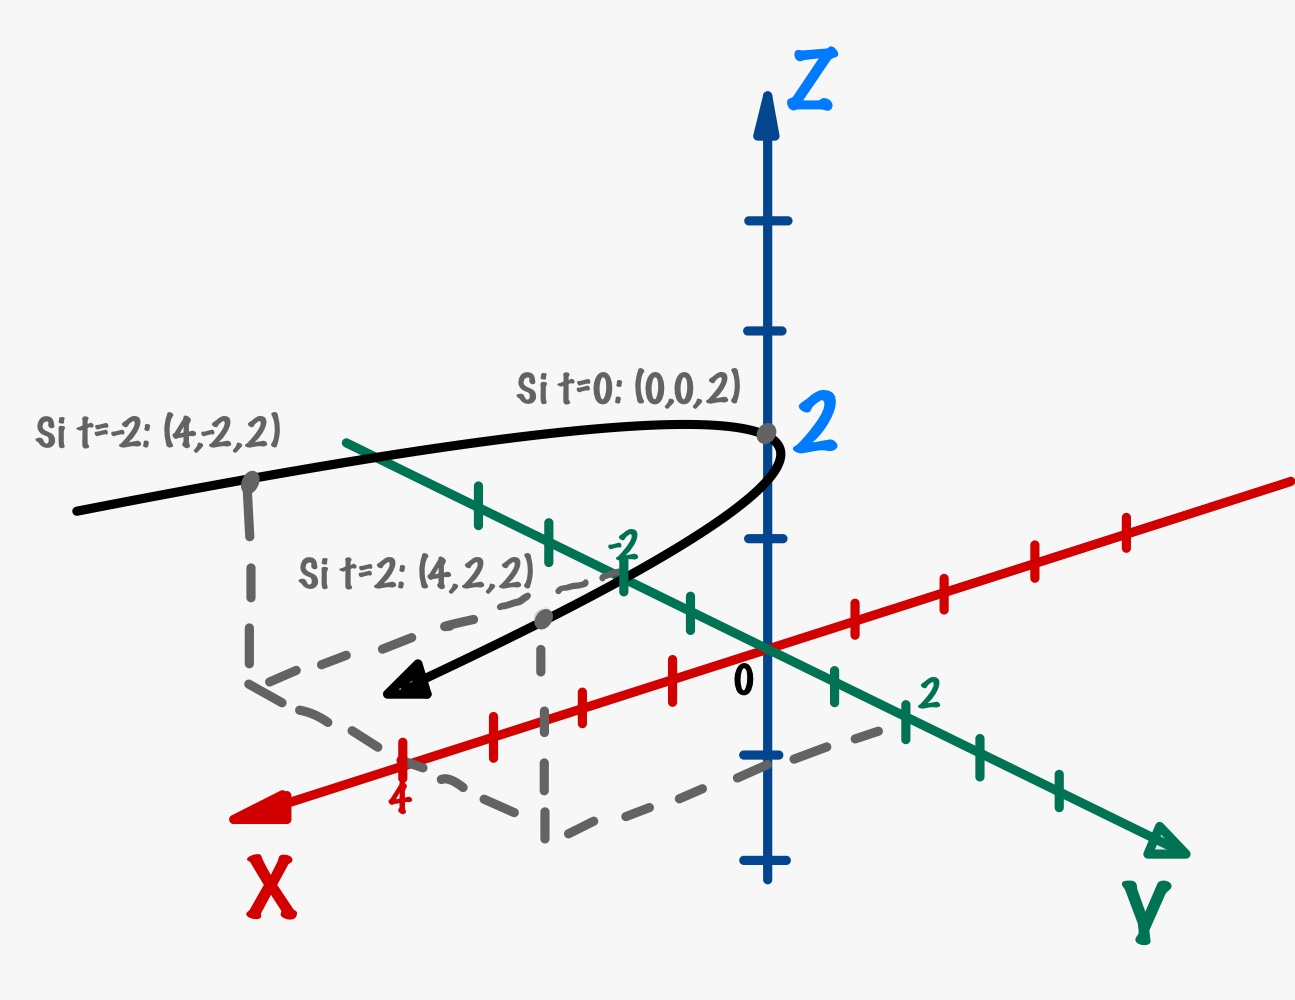
\includegraphics[width=0.7\textwidth]{./img/t2_ej3_1.jpeg}
  \end{figure}

\item $\vec{r(t)} = \cos{t}\hat{i}-\cos{t}\hat{j}+\sin{t}\hat{k}$
  \begin{figure}[H]
    \centering
    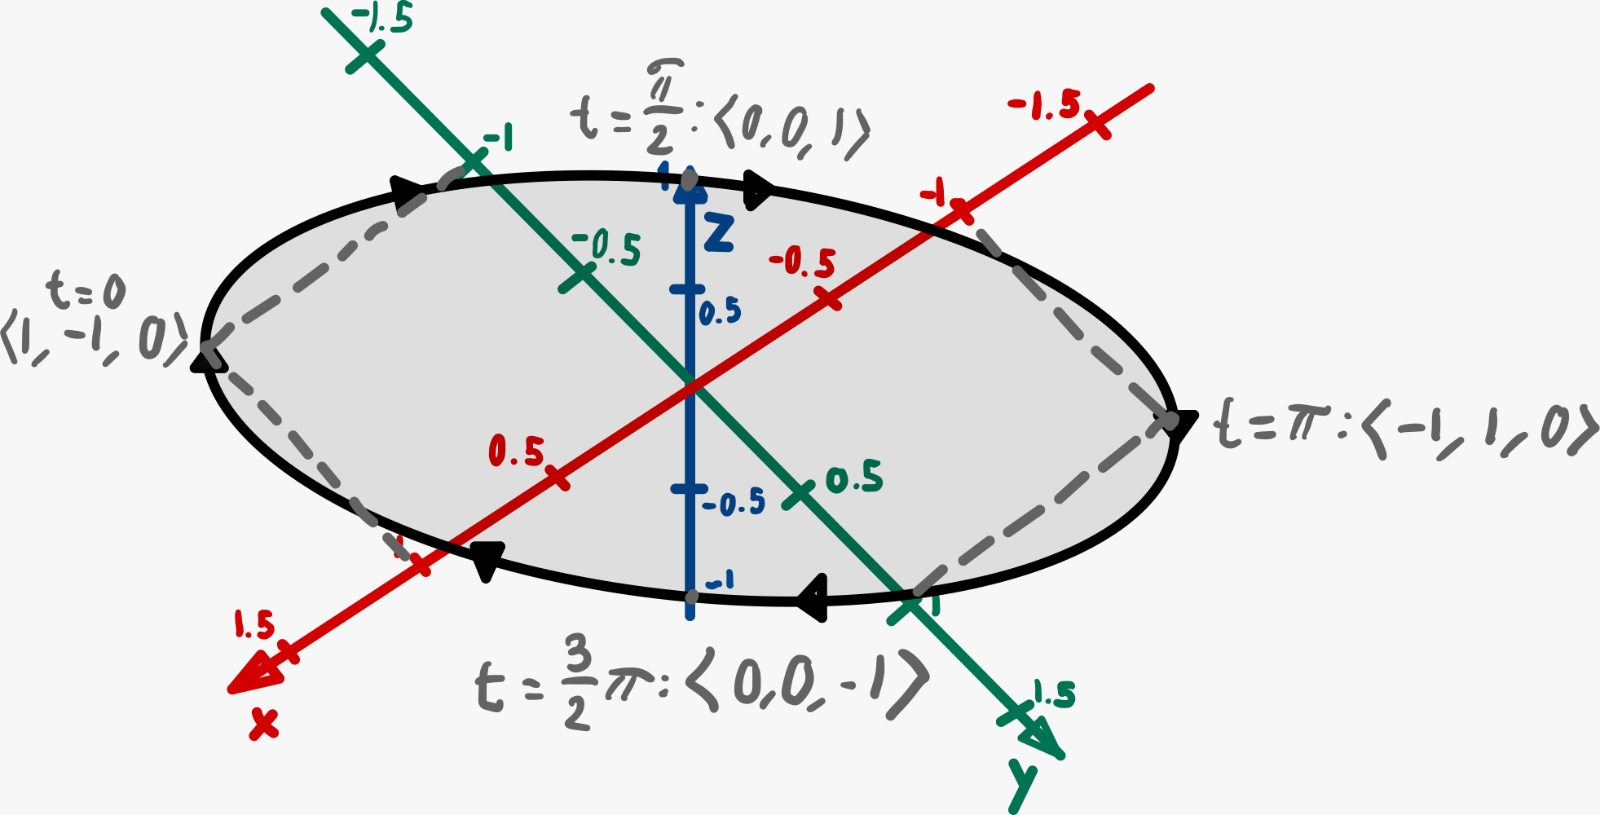
\includegraphics[width=0.9\textwidth]{./img/t2_ej3_2.jpeg}
  \end{figure}

\end{itemize}

% 4 -------------------------------------------------------------------------------------------------------------
\section{}
Proporcione las coordenadas del punto donde se intersectan la \textbf{hélice} $\vec{r(t)}=\sin{t}\hat{i}+\cos{t}\hat{j}+t\hat{k}$, y la \textbf{esfera} $x^2+y^2+z^2=5$.\\

Podemos observar que la ecuación de la función $\vec{r(t)}$ es la siguiente :
\[
\vec{r(t)}=\sin{t}\hat{i}+\cos{t}\hat{j}+t\hat{k} = (\sin{t},\cos{t}, t )\]
Y podemos obtener las ecuaciones paramétricas de $\vec{r(t)}$:
\[ x(t) =  \sin{t} \]
\[ y(t) =  \cos{t} \]
\[ z(t) =  t \]

Podemos usarlas para sustituirlas en la ecuación de la esfera:
 \begin{align*}
   x^2+y^2+z^2=5 \\
   (\sin^2{t}) + (\cos^2{t}) + t ^2 = 5 \\
   1+ t ^2 = 5 \\
   t ^2 = 4 \\
   \therefore t_1 = 2, ~ ~  t_2 = -2
 \end{align*}

 Y ya que tenemos el valor de t encontrar los puntos en que intersectan usando la función $\vec{r(t)}$ y estos serán los puntos de intersección:
\[
\vec{r(2)} = (\sin{2},\cos{2}, 2 )
\]
\[
\vec{r(-2)}= (\sin{-2},\cos{-2}, -2 )
\]
% 5 -------------------------------------------------------------------------------------------------------------
\section{}
Dibuje las proyecciones de la curva $\vec{r(t})=t\hat{i}+t\hat{j}+t^2\hat{k}$ sobre los planos $XY , XZ, YZ$. Utilice dichas proyecciones para hacer un esbozo de la curva.
  \begin{figure}[H]
    \centering
    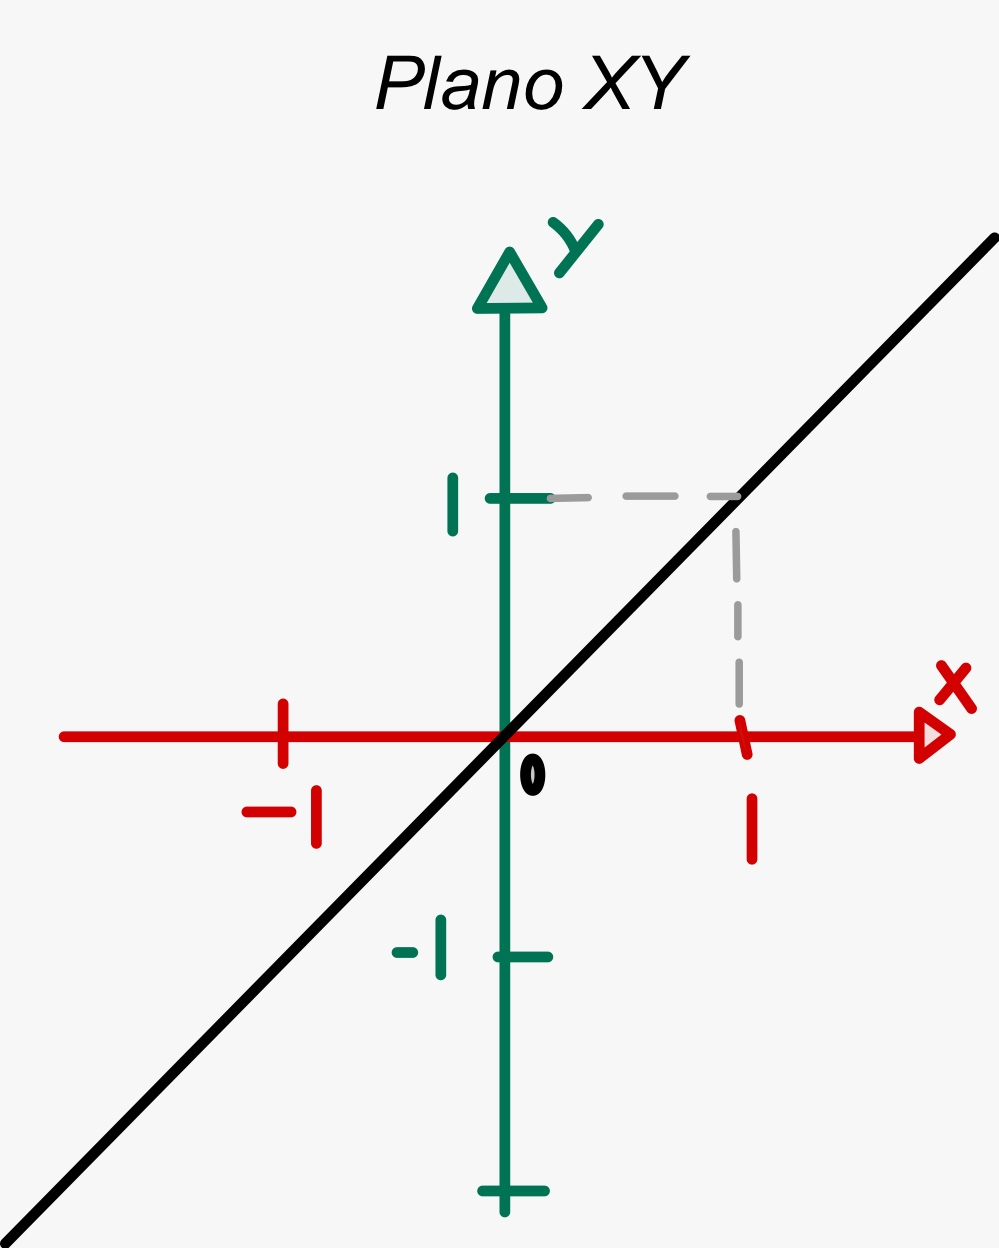
\includegraphics[width=0.35\textwidth]{./img/t2_ej5_xy.jpeg}
  \end{figure}
  \begin{figure}[H]
    \centering
    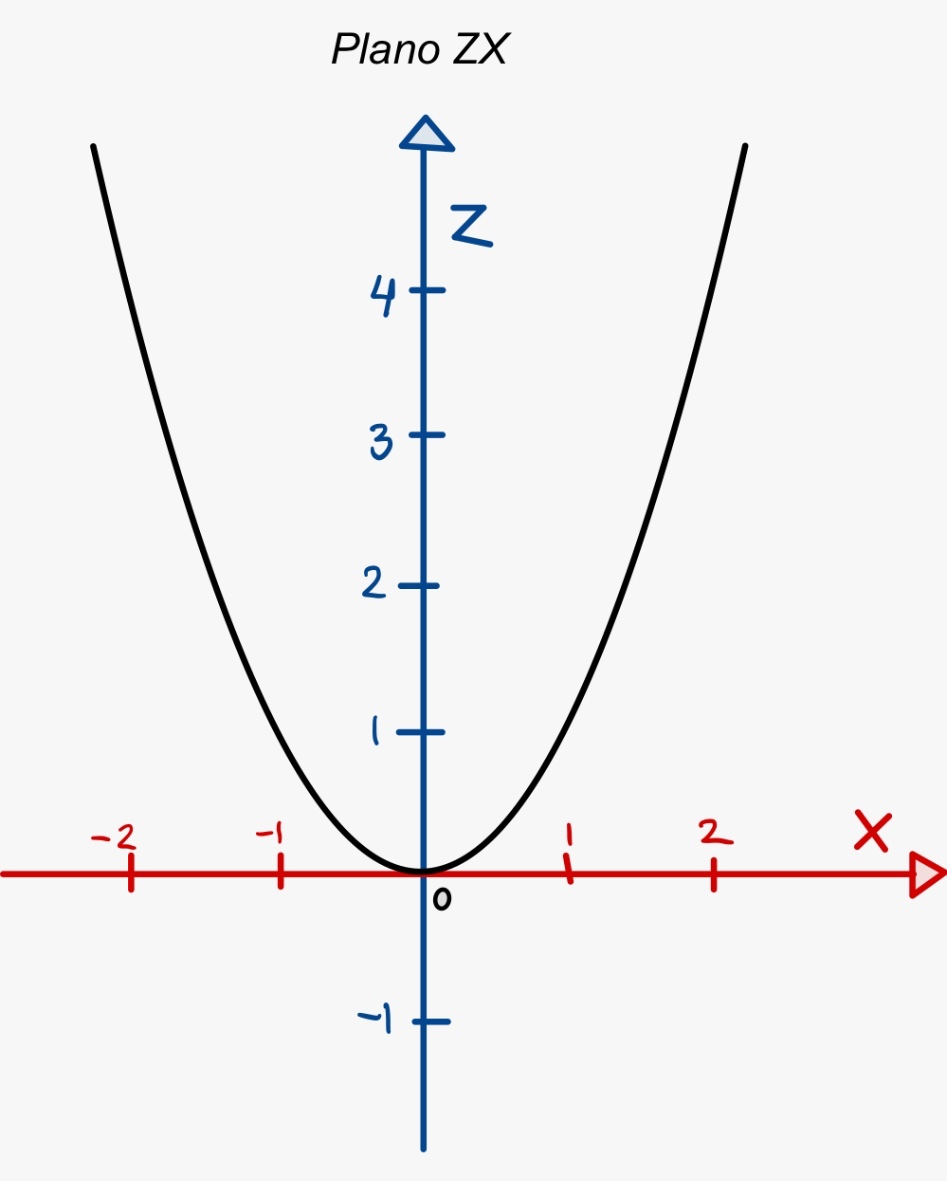
\includegraphics[width=0.45\textwidth]{./img/t2_ej5_zx.jpeg}
  \end{figure}
  \begin{figure}[H]
    \centering
    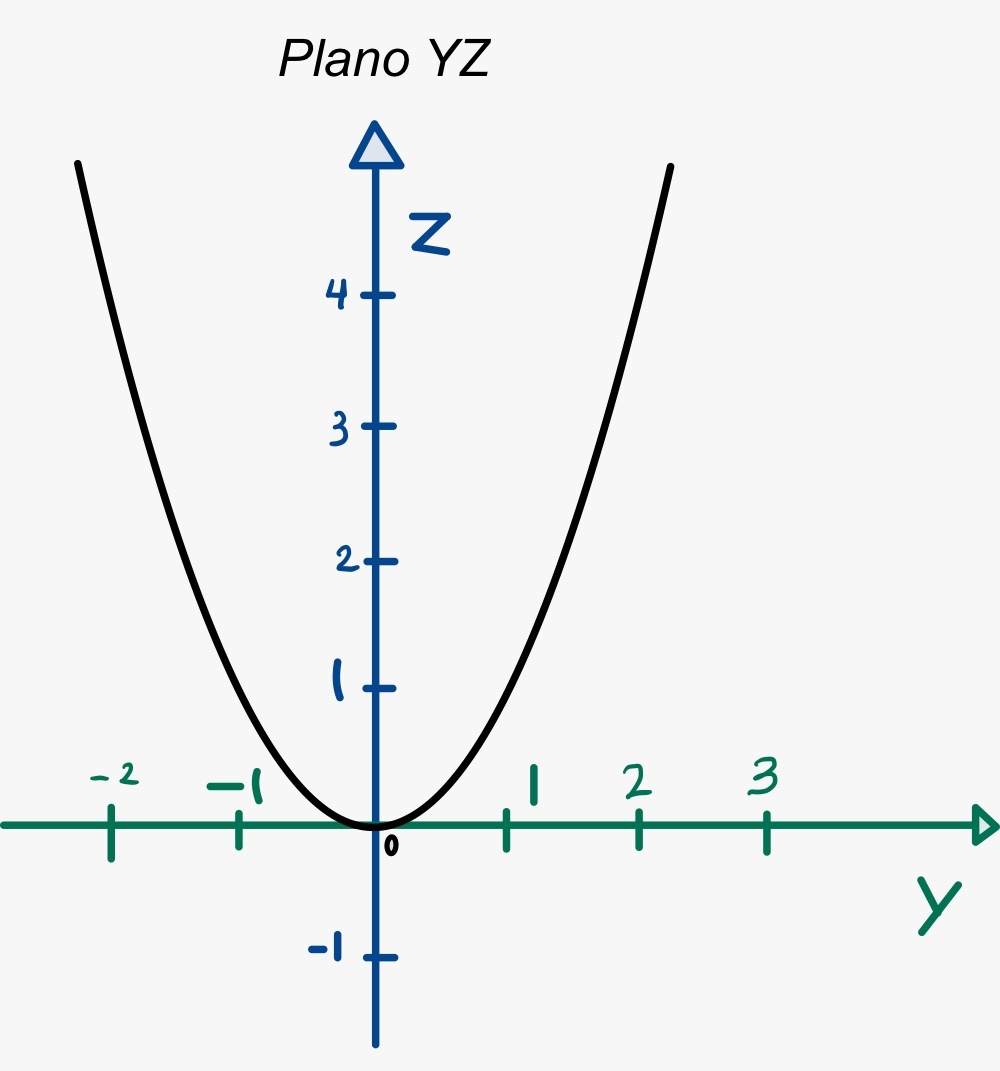
\includegraphics[width=0.45\textwidth]{./img/t2_ej5_yz.jpeg}
  \end{figure}
  \begin{figure}[H]
    \centering
    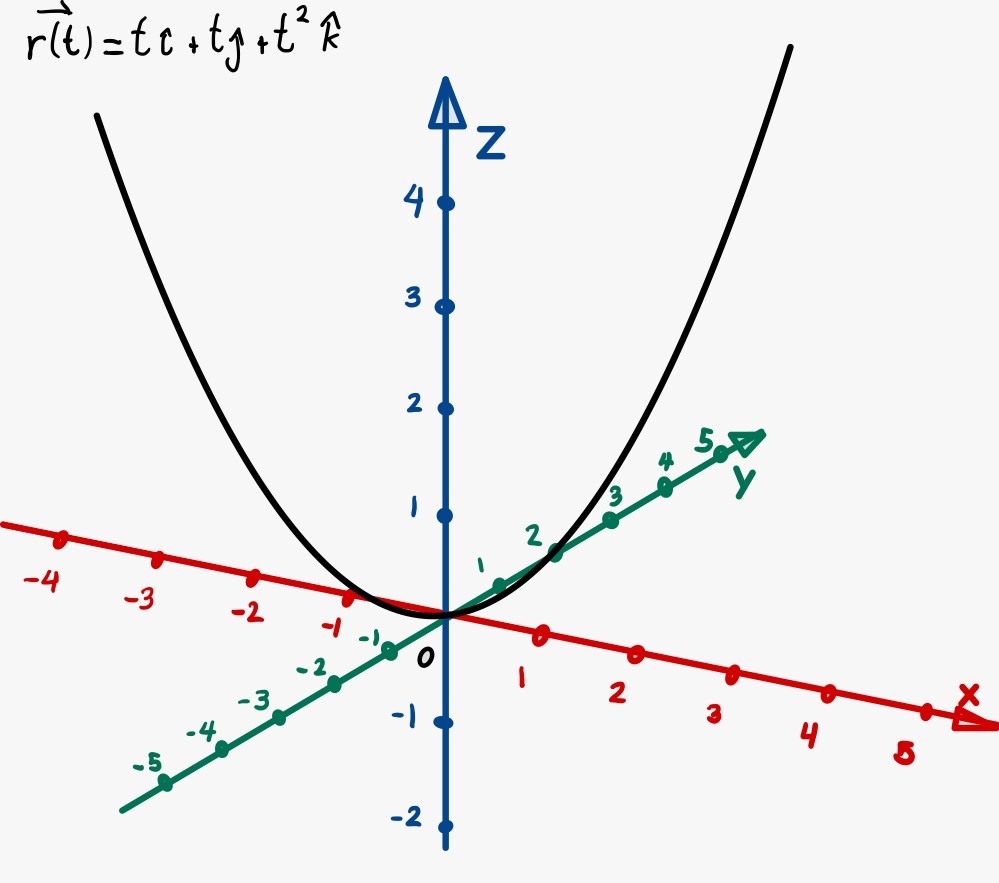
\includegraphics[width=0.9\textwidth]{./img/t2_ej5_curva.jpeg}
  \end{figure}

% 6 -------------------------------------------------------------------------------------------------------------
\section{}
Las trayectorias de dos partículas están dadas por las siguientes funciones vectoriales:
\begin{itemize}[format=\textbf]

\item $\vec{r_1(t)}=t\hat{i}+t^2\hat{j}+t^3\hat{k}$

\item $\vec{r_2(t)}=(1+2t,1+6t,1+14t)$

\end{itemize}
¿Chocarán las partículas? ¿En qué punto? ¿Se cortarán las trayectorias?

1. Para saber si las partículas colisionarán debemos encontrar una t para la cual $\vec{r_1(t)} = \vec{r_2(t)}$.Así, tomaremos las ecuaciones paramétricas de $r_1$:
\[ x_1 = t\]
\[ y_1 = t^2\]
\[ z_1 = t^3\]
Y las de $\vec{r_2(t)}$
\[ x_2 = 1+2t\]
\[ y_2 = 1+6t\]
\[ z_2 = 1+14t\]
e igualaremos primero $x_1 = x_2$
 \begin{align*}
   x_1 = x_2 \\
   t = 1+2t \\
   t=-1
 \end{align*}
 y veremos si $t=-1$ es solución para $y_1 = y_2$
 \begin{align*}
   y_1 = y_2 \\
   t^2 =  1+6t \\
   t^2 -6t -1 = 0 \\
   (-1)^2 - 6 (-1) -1 = 1 +6 -1 = 6 \neq 0
 \end{align*}

$ \therefore $ Ya que el sistema de ecuaciones no tiene una solución que satisfaga todas las igualdades para las componentes de $r_1 $y$ r_2$ , las partículas \textbf{no colisionan} en ningún momento t y en ningún punto.\\

 2. Para ver si las trayectorias se cortan, debemos saber si existe una t para $\vec{r_1(t)}$ y una s para $\vec{r_2(s)}$ tales que $\vec{r_1(t)} = \vec{r_2(s)}$.
 Para esto, haremos un sistema de ecuaciones, primero tomemos las ecuaciones paramétricas de $\vec{r_1(t)}$.
 \[ x_1 = t\]
\[ y_1 = t^2\]
\[ z_1 = t^3\]
y las de $\vec{r_2(s)}$.
\[ x_2 = 1+2s\]
\[ y_2 = 1+6s\]
\[ z_2 = 1+14s\]
Igualamos las componentes x.
\begin{align*}
   x_1 = x_2 \\
   t =  1+2s \\
\end{align*}
Y las componentes y.
\begin{align*}
   y_1 = y_2 \\
   t^2 =  1+6s \\
\end{align*}
Ahora con el sistema de ecuaciones
\begin{align*}
   (1) t =  1+2s \\
   (2) t^2 =  1+6s \\
\end{align*}
Podemos sustituir t en (2)
\begin{align*}
   t^2 =  1+6s \\
   (1+2s)^2= 1+6s \\
   1+4s+4s^2 = 1 + 6s \\
   4s^2 + -2s = 0 \\
   (2s)(2s-1) = 0 \\
   \therefore s_1 = 0 \\
   s_2 = \frac{1}{2} \\
\end{align*}
Ahora sustituiremos en (1)
\\
Para $s_1$ :
\begin{align*}
    t =  1+2s \\
   t_1 = 1 + 2 (0) = 1
\end{align*}
Y para $s_2$ :
\begin{align*}
    t =  1+2s \\
   t_2 = 1 + 2 \left(\frac{1}{2} \right) = 2
\end{align*}

Ya que tenemos estas soluciones las probamos en 
\begin{align*}
   z_1 = z_2 \\
   t^3 =  1+14s \\
\end{align*}
Con $s_1, t_1$

\begin{align*}
  t^3 =  1+14s \\
  (1)^3 =  1+14(0)  \\
  1 =  1  \\
\end{align*}
Se satisface. \\
Con $s_2, t_2$

\begin{align*}
  t^3 =  1+14s \\
  2^3 =  1+14 \left( \frac{1}{2} \right) \\
  8  =  1 + \left(\frac{14}{2} \right) \\
   8  =  8 \\
\end{align*}
Se satisface.

Por lo tanto, las trayectorias se intersectan en dos puntos.\\
Punto 1: $t=1 , s=0$ :
\item $\vec{r_1(1)}=1\hat{i}+1^2\hat{j}+1^3\hat{k} = (1, 1, 1) $

\item $\vec{r_2(0)}=(1+2 \cdot 0,1+6 \cdot 0,1+14 \cdot 0) = (1, 1, 1) $\\
  Entonces el primer punto donde intersectan las trayectorias es (1, 1, 1) \\ \\
 Punto 2: $t=2 , s=\frac{1}{2}$:
  \item $\vec{r_1(2)}=2\hat{i}+2^2\hat{j}+2^3\hat{k} = (2, 4, 8) $

\item $\vec{r_2(\frac{1}{2})}=(1+2 \cdot \frac{1}{2} ,1+6 \cdot \frac{1}{2},1+14 \cdot \frac{1}{2}) = (2, 4, 8) $\\
  Entonces el segundo punto donde intersectan las trayectorias es (2, 4, 8) \\
$ \therefore $ Las trayectorias \textbf{sí se cortan} en dos puntos.
% 7 -------------------------------------------------------------------------------------------------------------
\section{}
Proporcione las coordenadas del punto sobre la curva $\vec{r(t)}=(2\cos{t},2\sin{t},\mathrm{e}^t)$, con $t \in [0,\pi]$, donde la \textbf{recta tangente} a la curva es paralela al plano $\sqrt{3}x+y=1$. \\

Sea $P_0=(x_0,y_0,z_0)$ el punto sobre la curva $\vec{r(t)}=(2\cos{t},2\sin{t},\mathrm{e}^t)$ cuya recta tangente es paralela al plano $\sqrt{3}x+y=1$ para alguna $t_0 \in [0,\pi]$, i.e., $r(t_0)=P_0$.

Nótese que el vector director de la recta tangente a la curva $\vec{r(t)}$ en $P_0$, está dado por $\vec{r'(t_0)}=(-2\sin{t_0},2\cos{t_0},\mathrm{e}^{ t_0})$. Además, el vector normal del plano es $\vec{n}=(\sqrt{3},1,0)$.

Dado que la recta debe ser paralela al plano $\sqrt{3}x+y=1$, se tiene que $\vec{n}$ y $\vec{r'(t_0)}$ son ortogonales, es decir, su producto punto es cero

\begin{align*}
   \vec{n} \cdot \vec{r'(t_0)} &= 0 \\
  (\sqrt{3},1,0) \cdot (-2\sin{t_0},2\cos{t_0},\mathrm{e}^{ t_0}) &=0 \\
  -2\sqrt{3}\sin{t_0} + 2\cos{t_0} + 0 &= 0 \\
  -\sqrt{3}\sin{t_0} + \cos{t_0} &= 0 \\
  \sqrt{3}\sin{t_0} &= \cos{t_0} \\
  \tan{t_0} &= \frac{1}{\sqrt{3}} \\
  \arctan{t_0} &= \frac{\sqrt{3}}{3}\\
  t_0 &= \frac{\pi}{6}
\end{align*}

Así, se tiene que

\begin{align*}
  P_0 = r(t_0) = r\left(\frac{\pi}{6}\right) &= \left(2\cos{\frac{\pi}{6}},2\sin{\frac{\pi}{6}},\mathrm{e}^{\frac{\pi}{6}}\right) \\
  &= \left(2\cdot \frac{\sqrt{3}}{2},2\cdot \frac{1}{2},\mathrm{e}^{\frac{\pi}{6}}\right) \\
  &= \left(\sqrt{3},1,e^{\frac{\pi}{6}}\right)
\end{align*}

$\therefore \left(\sqrt{3},1,e^{\frac{\pi}{6}}\right)$ son las coordenadas del punto sobre la curva $\vec{r(t)}=(2\cos{t},2\sin{t},\mathrm{e}^t)$, con $t \in [0,\pi]$, donde la \textbf{recta tangente} a la curva es paralela al plano $\sqrt{3}x+y=1$.

% 8 -------------------------------------------------------------------------------------------------------------
\section{}
Proporcione las coordenadas del punto donde se intersectan las curvas:
\begin{itemize}[format=\textbf]

\item $\vec{r_1(t)}=(t,1-t,3+t^2)$

\item $\vec{r_2(s)}=(3-s,s-2,s^2)$

\end{itemize}

Ademas proporcione el  ́angulo de intersección de ambas trayectorias. \\

Primero, para encontrar el punto donde se intersectan las curvas, daremos las ecuaciones paramétricas de $\vec{r_1(t)}$:
\[ x_1 = t\]
\[ y_1 = 1-t\]
\[ z_1 = 3+t^2\]
y de $\vec{r_2(s)}$:
\[ x_2 = 3-s\]
\[ y_2 = s-2\]
\[ z_2 = s^{2} \]

Igualaremos las componentes de x:
\begin{align*}
   x_1 = x_2 \\
   t =  3-s \\
\end{align*}
Y las de z:
\begin{align*}
   z_1 = z_2 \\
   3+t^2  =  s^{2} \\
\end{align*}
Y tenemos un sistema de ecuaciones:
\begin{align*}
  (1) t =  3-s \\
  (2) 3+t^2  =  s^{2}
\end{align*}
Sustituimos (1) en (2).
\begin{align*}
   3+(3-s)^2  =  s^{2} \\
   3+9-6s+s^2  =  s^{2} \\
   12 -6s =  0 \\
   s = 2
\end{align*}
Y con sustituimos s = 2 en (1).
\begin{align*}
   t =  3-s \\
  t = 3-2 = 1 
\end{align*}

Vemos que satisface la igualdad de las componentes de y:
\begin{align*}
   1-t = s-2 \\
   1-1  = 2-2 \\
   0 = 0
\end{align*}
Se satisface.\\
Por lo tanto veremos que el punto de intersección será donde $t=1, s=2$: \\
\item $\vec{r_1(1)}=(1,1-1,3+1^2) = (1, 0, 4)$

\item $\vec{r_2(2)}=(3-2,2-2,2^2) = (1, 0, 4)$ \\
  
  $\therefore$ El punto donde se intersectan las curvas es \textbf{(1, 0, 4)}
  \\
  
  Ahora, el ángulo entre dos curvas que se intersectan se define como el ángulo entre las dos tangentes de las dos curvas en el punto de intersección.\\
  Para esto necesitamos calcular los  vector tangente a las curvas mediante sus derivadas evaluadas en el punto de intersección.
\begin{align*}
    \vec{r_1'(t)} = \left( \frac{d}{dt} t, \frac{d}{dt}  (1-t), \frac{d}{dt} (3+t^2) \right) =  (1, -1, 2t)
\end{align*}

\begin{align*}
    \vec{r_2'(s)} = \left( \frac{d}{ds} (3-s),\frac{d}{ds} (s-2),\frac{d}{ds}(s^2)  \right) = (-1, 1, 2s) 
\end{align*}

Ahora evaluamos $\vec{r_1'(t)}$ en t =1 ya que es el valor que da el punto de intersección y tenemos los vectores tangentes:
\begin{align*}
    \vec{r_1'(1)} =  (1, -1, 2(1))  =(1, -1, 2)
\end{align*}
y  $\vec{r_2'(s)}$ en s= 2: 
\begin{align*}
  \vec{r_2'(2)} = (-1, 1, 2(2)) = (-1, 1, 4)
\end{align*}
Ya que tenemos estos vectores, el ángulo entre ellos está dado por :
\[
\theta = cos^{-1 }\left(\frac{\vec{u} \cdot \vec{v}}{||\vec{u}|| ||\vec{v}||}\right)
\]
Entonces
\begin{align*}
  \theta &= cos^{-1 }\left(\frac{\vec{u} \cdot \vec{v}}{||\vec{u}|| ||\vec{v}||}\right) = cos^{-1 }\left(\frac{(1, -1, 2) \cdot (-1, 1, 4)}{||(1, -1, 2)|| ||(-1, 1, 4)||}\right) \\
  &=  cos^{-1 }\left(  \frac{1 \cdot -1 + -1 \cdot 1 + 2 \cdot 4}{\sqrt{1^2 + (-1)^2 + 2^2} \cdot \sqrt{(-1)^2 + 1^2 + 4^2}} \right) \\
  &=  cos^{-1 }\left( \frac{-1  -1 + 8}{\sqrt{1 + 1 + 4} \cdot \sqrt{1 + 1 + 16}} \right)  =  cos^{-1 }\left( \frac{6}{\sqrt{6} \cdot \sqrt{18}}\right) \\
  &\approx 54.735 ^\circ 
\end{align*}

$\therefore$ El \textbf{ángulo de intersección} de ambas trayectorias es $54.73561 ^\circ$ 


% 9 -------------------------------------------------------------------------------------------------------------
\section{}
Determine la \textbf{longitud de curva} para las siguientes curvas:
\begin{itemize}[format=\textbf]

\item $\vec{r(t)}=\left(2t,t^2,\frac{t^3}{3}\right)$, para $t \in [0,1]$

\item $\vec{r(t)}=\left(\cos{t},\sin{t},\ln{\cos{t}}\right)$, para $t \in \left[0,\frac{\pi}{4}\right]$

\end{itemize}

Sabemos que la fórmula para encontrar la longitud de arco es $$ L = \int_a^b ||r'(t)||dt $$

Por lo que, en $\vec{r(t)}=\left(2t,t^2,\frac{t^3}{3}\right)$, para $t \in [0,1]$; tenemos que,
\begin{align*}
  \vec{r'(t)} = \left( 2,2t,t^2 \right)
\end{align*}
Entonces,
\begin{align*}
  ||\vec{r'(t)}|| &= \sqrt{(2)^2+(2t)^2+(t^2)^2}\\
  &=  \sqrt{4+4t^2+t^4}\\
  &= \sqrt{(t^2+2)^2}\\
  &= t^2+2
\end{align*}
Así
\begin{align*}
  \int_0^1 (t^2+2)~ dt &= \frac{t^3}{3}+2t \Bigg|_0^1 \\
  &= \left(\frac{1}{3}+2 \right) - \left(\frac{0}{3}+0\right) \\
  &= \frac{7}{3}
\end{align*}
$\therefore L=\frac{7}{3}$ es la \textbf{longitud de curva} en $\vec{r(t)}=\left(2t,t^2,\frac{t^3}{3}\right)$, para $t \in [0,1]$. \\

Ahora, en $\vec{r(t)}=\left(\cos{t},\sin{t},\ln{\cos{t}}\right)$, para $t \in \left[0,\frac{\pi}{4}\right]$; tenemos que,
\begin{align*}
  \frac{d}{dt} \ln{\cos{t}} &= \frac{1}{\cos{t}} \cdot \frac{d}{dt} \cos{t}\\
  &=  \frac{1}{\cos{t}} \cdot -\sin{t}\\
  &= -\tan{t} \\
  \therefore \vec{r'(t)} = \left( -\sin{t},\cos{t}, -\tan{t}\right) \\
\end{align*}
Entonces, 
\begin{align*}
  ||\vec{r'(t)}|| &= \sqrt{(-\sin{t})^2+(\cos{t})^2+(-\tan{t})^2} \\
  &= \sqrt{(\sin^2{t}+\cos^2{t})+\tan^2{t}} \\
  &= \sqrt{1+\tan^2{t}} \\
  &= \sqrt{\sec^2{t}} \\
  &= \sec{t}
\end{align*}
Así,
\begin{align*}
  \int_0^{\frac{\pi}{4}} \sec{t}~dt &= \ln{|\sec{t}+\tan{t}|} \Bigg|_0^{\frac{\pi}{4}} \\
  &= \left[ \ln{\Bigg|\sec{\frac{\pi}{4}}+\tan{\frac{\pi}{4}}\Bigg|} \right]
  -\left[ \ln{\Bigg|\sec{0}+\tan{0}\Bigg|} \right] \\
  &= \left[ \ln{|\sqrt{2}+1|} \right]
  -\left[ \ln{|1+0|} \right] \\
  &= \ln{|\sqrt{2}+1|}
  - \ln{1} \\
  &= \ln{|\sqrt{2}+1|}
  - 0 \\
  &= \ln{|\sqrt{2}+1|}\\
\end{align*}
$\therefore L=\ln{|\sqrt{2}+1|}$ es la \textbf{longitud de curva} en  $\vec{r(t)}=\left(\cos{t},\sin{t},\ln{\cos{t}}\right)$, para $t \in \left[0,\frac{\pi}{4}\right]$.\\

% 10 -------------------------------------------------------------------------------------------------------------
\section{}
Reparametrice la siguiente curva (respecto a la longitud de arco medida desde el punto donde $t = 0$), en la dirección en que $t$ se incrementa.
$$ \vec{r(t)}=(2t)\hat{i}+(1-3t)\hat{j}+(5+4t)\hat{k}$$
Sea s(t) la función longitud de arco, entonces podríamos determinar t como una función de s: t = t(s). Entonces la curva se puede reparametrizar en términos de s al sustituir a t en su lugar t: r = r(t(s)).

\begin{align*}
  \frac{ds}{dt} &= || r'(t)|| = \left|\left| \left( \frac{d}{dt} (2t), \frac{d}{dt} (1-3t),   \frac{d}{dt} (5+4t)  \right) \right| \right| \\
  &=  \left|\left| \left(2, -3,  4  \right) \right| \right| \\
  &= \sqrt{2^2+ (-3^2) + 4^2} = \sqrt{4+ 9 + 16} = \sqrt{29}
\end{align*}

Por tanto, $t = \frac{s}{\sqrt{29}}$ y la reparametrización requerida se obtiene al sustituir el valor de t:

$ \vec{r(t(s))} = (2(\frac{s}{\sqrt{29}}))\hat{i}+(1-3( \frac{s}{\sqrt{29}}))\hat{j}+(5+4( \frac{s}{\sqrt{29}}))\hat{k} $
\end{document}

